\appendix
\addappheadtotoc
\appendixpage

\chapter{Planificaci\'on de Actividades}
\label{appen:planificacion}

\newpage
\section[WBS]{Work Breakdown Structure}
\label{section:wbs}

En las siguientes p\'aginas se muestra la estimaci\'on del esfuerzo estimado para el proyecto \emph{V.I.Pe.R.}:

\begin{table}[H]
  \centering
  \begin{tabular}{|l|m{5cm}|c|c|c|}\hline
    {\bf Fase} & {\bf Tarea} & {\bf Esfuerzo} & {\bf Hrs. Equipo} & {\bf Hrs. Hombre}\\\hline
    \multirow{4}{*}{Inicio} & Decisi\'on aplicaci\'on                & 3 & 12 & 48\\\cline{2-5}
           & Pruebas de robot                   & 3 & 12 & 48\\\cline{2-5}
           & Definici\'on software de desarrollo  & 2 & 12 & 48\\\cline{2-5}
           & Definici\'on nombre pre-empresa y producto & 2 & 8 & 32\\\hline
    \multirow{7}{*}{Elaboraci\'on} & Propuesta T\'ecnica           & 3 & 12 & 48\\\cline{2-5}
                & Toma de requisitos          & 5 & 20 & 80\\\cline{2-5}
                & Especificaci\'on casos de uso & 4 & 16 & 64\\\cline{2-5}
                & Identificaci\'on de riesgos   & 5 & 20 & 80\\\cline{2-5}
                & Mitigaci\'on de riesgos       & 5 & 20 & 80\\\cline{2-5}
                & P\'agina web                  & 3 & 12 & 48\\\cline{2-5}
                & Plan de proyecto            & 4 & 16 & 64\\\hline
    \multirow{5}{*}{Desarrollo} & Dise\~no de Interfaz                            & 5 & 20 & 100\\\cline{2-5}
               & Programaci\'on de Casos de Uso/Requerimientos   & 5 & 20 & 100\\\cline{2-5}
               & Testing                                       & 3 & 12 & 60\\\cline{2-5}
               & Feedback                                      & 3 & 12 & 60\\\cline{2-5}
               & Algo de nivel 3?!                             &   &    &\\\hline
                & {\bf Total}                 & 55 & 224 & 960\\\hline
  \end{tabular}
  \label{tab:wbs}
  \caption[~Tabla WBS]{Divisi\'on de trabajo, seg\'un modelo utilizado, por esfuerzo.}
\end{table}

\newpage
%CARTA GANTT
\section{Carta Gantt}
\label{appen:gantt}

%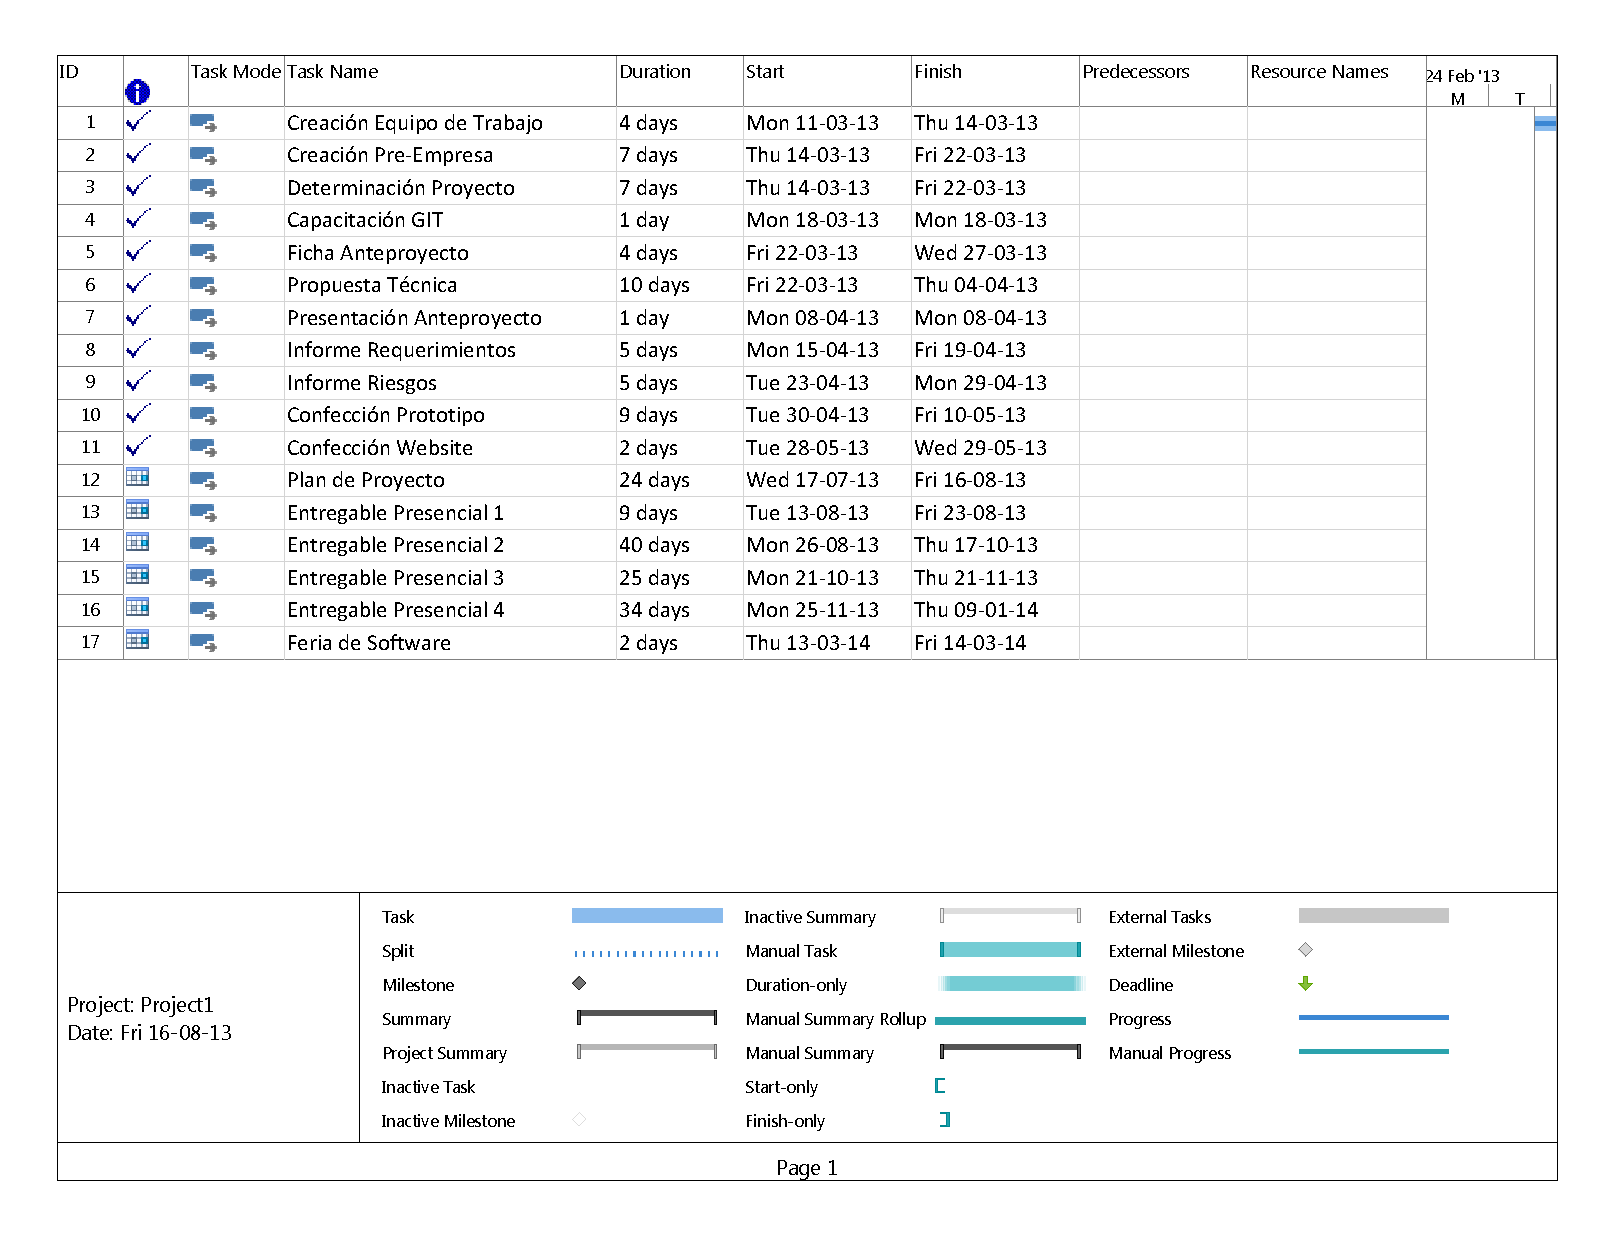
\includepdf[pagecommand={\section{Carta Gantt}},scale=0.7,pages=1,angle=-90,addtotoc={37,section,1,{Carta Gantt},appen:gantt}]{./pic/gantt.pdf}
%\includepdf[scale=0.7,pages=2-3,angle=-90,pagecommand={}]{./pic/gantt.pdf}

\begin{figure}[H]
\centering
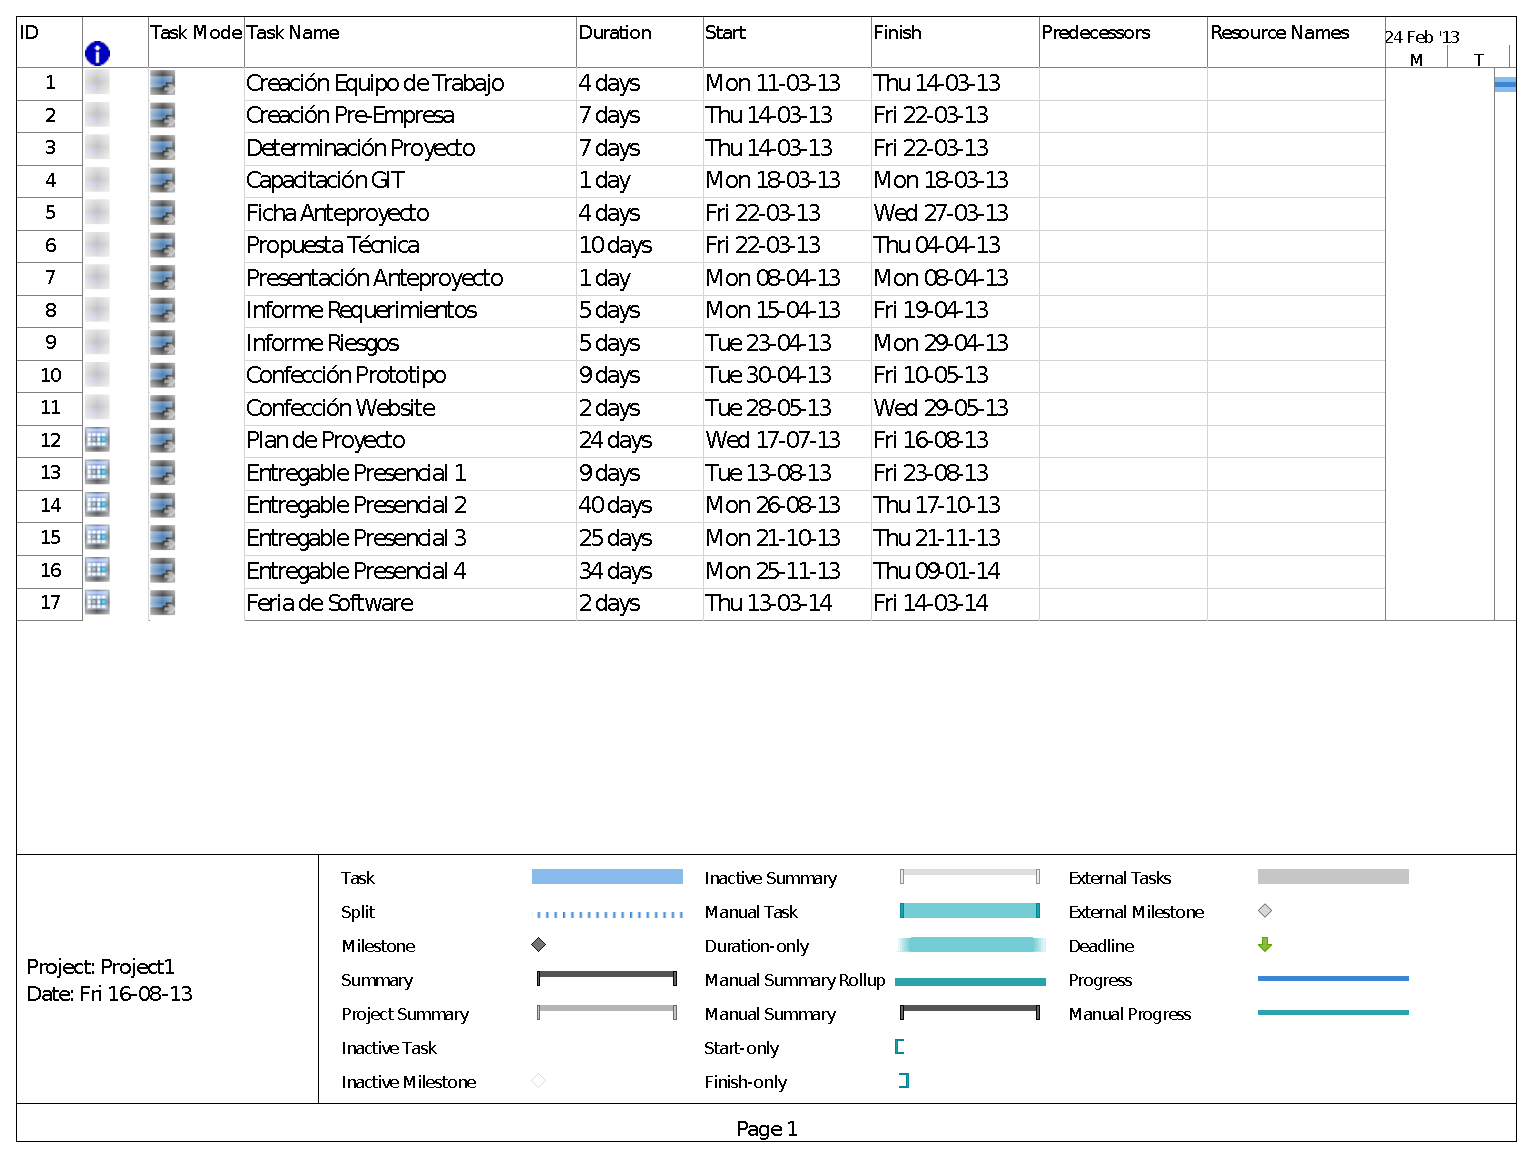
\includegraphics[angle=-90,scale=0.7]{gantt1.eps}
\label{fig:gantt1}
\end{figure}

\begin{figure}[htbp!]
\centering
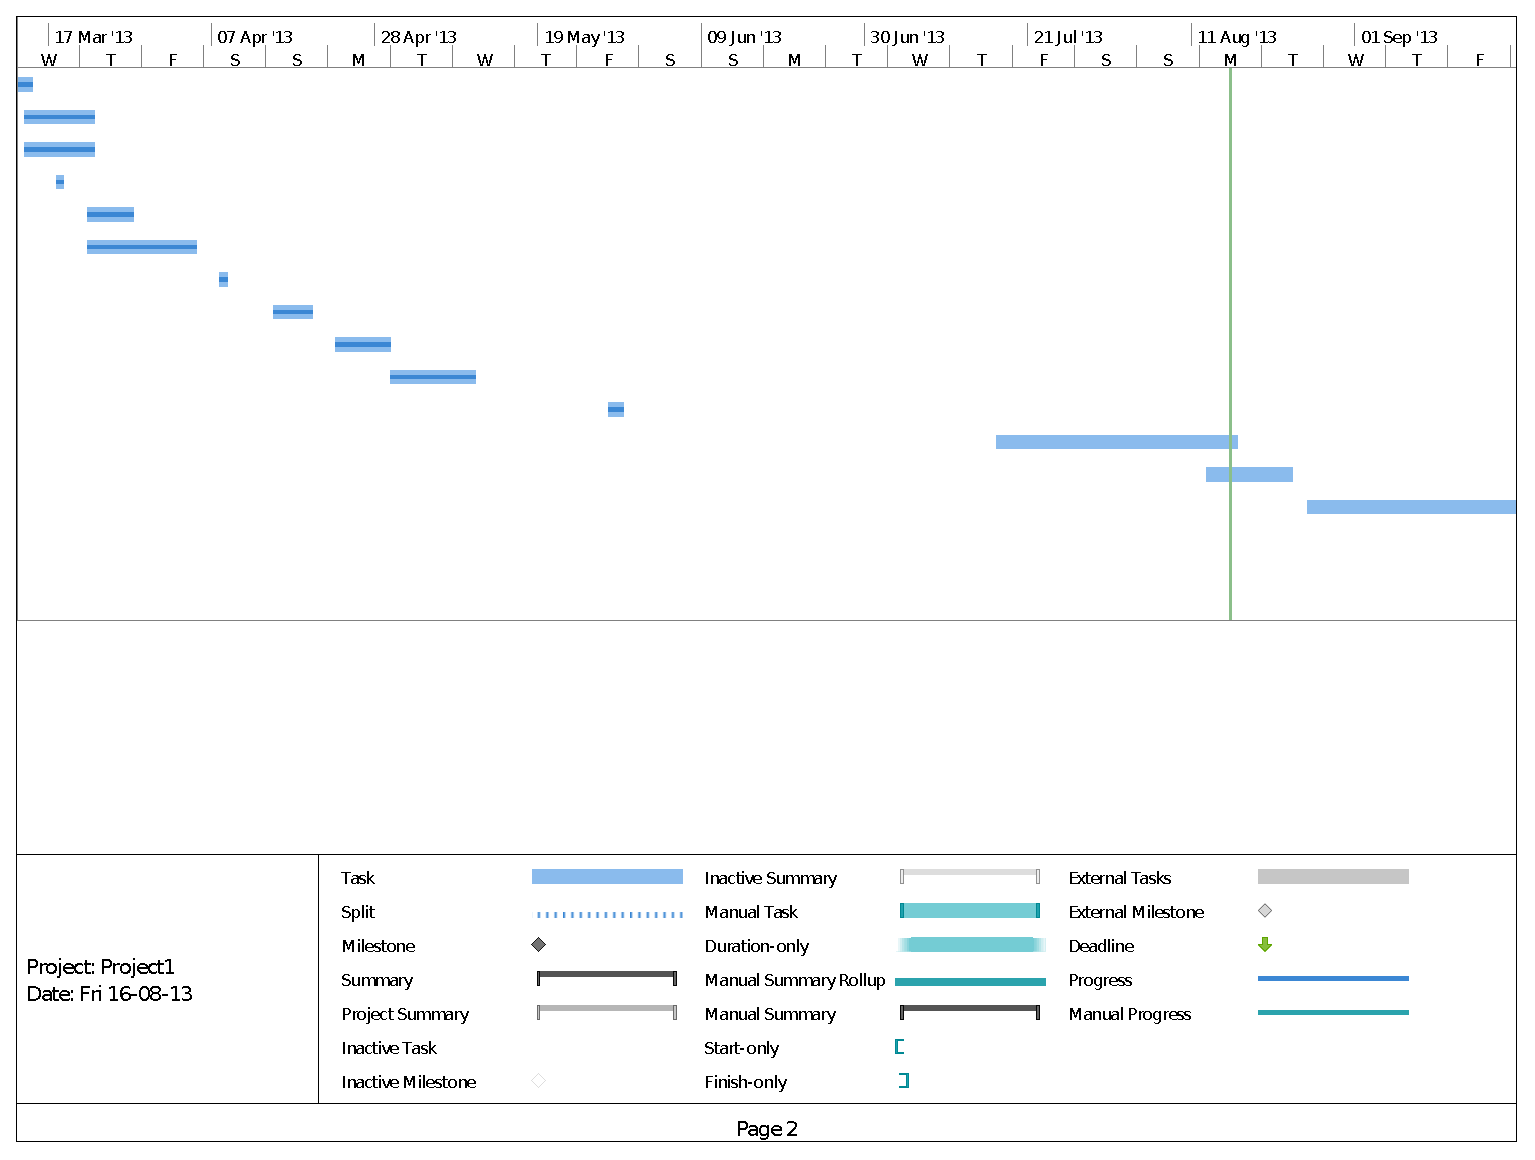
\includegraphics[angle=-90,scale=0.7]{gantt2.eps}
\label{fig:gantt1}
\end{figure}

\begin{figure}[htbp!]
\centering
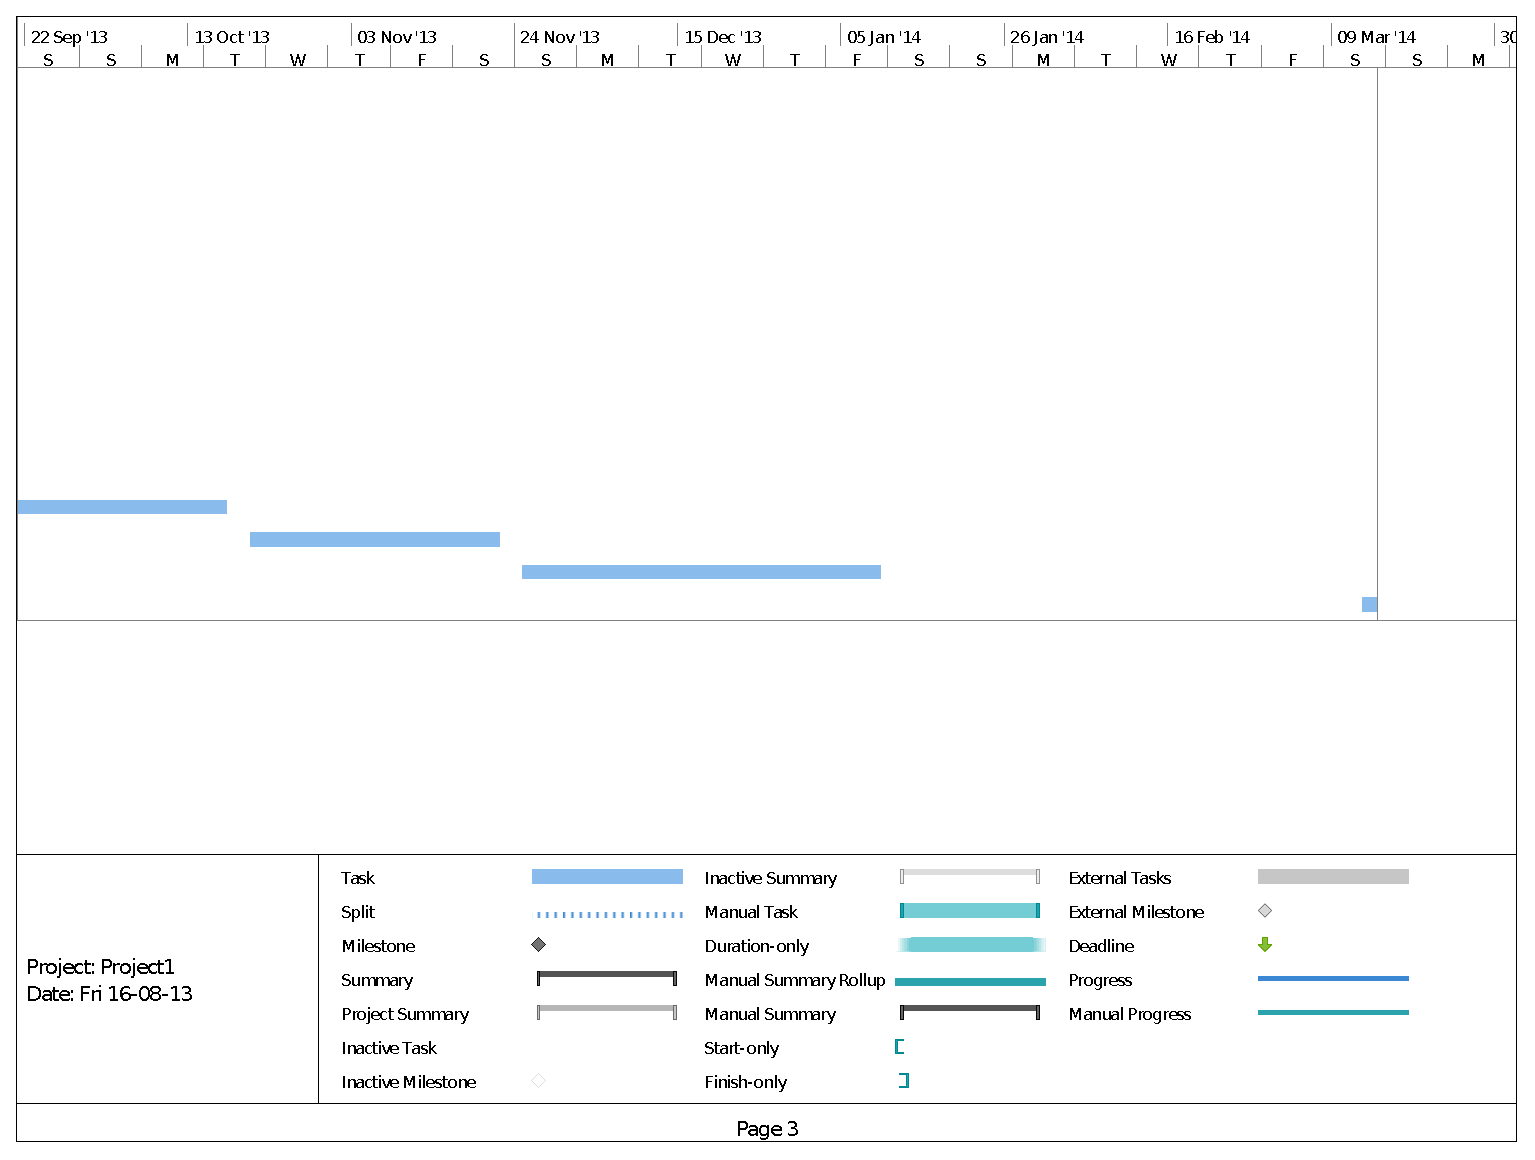
\includegraphics[angle=-90,scale=0.7]{gantt3.eps}
\label{fig:gantt1}
\end{figure}
